
\subsection{Multi-Label Object Classification}
% Describe here the CNN architecture.


\begin{figure*}[!h]
     \begin{center}
       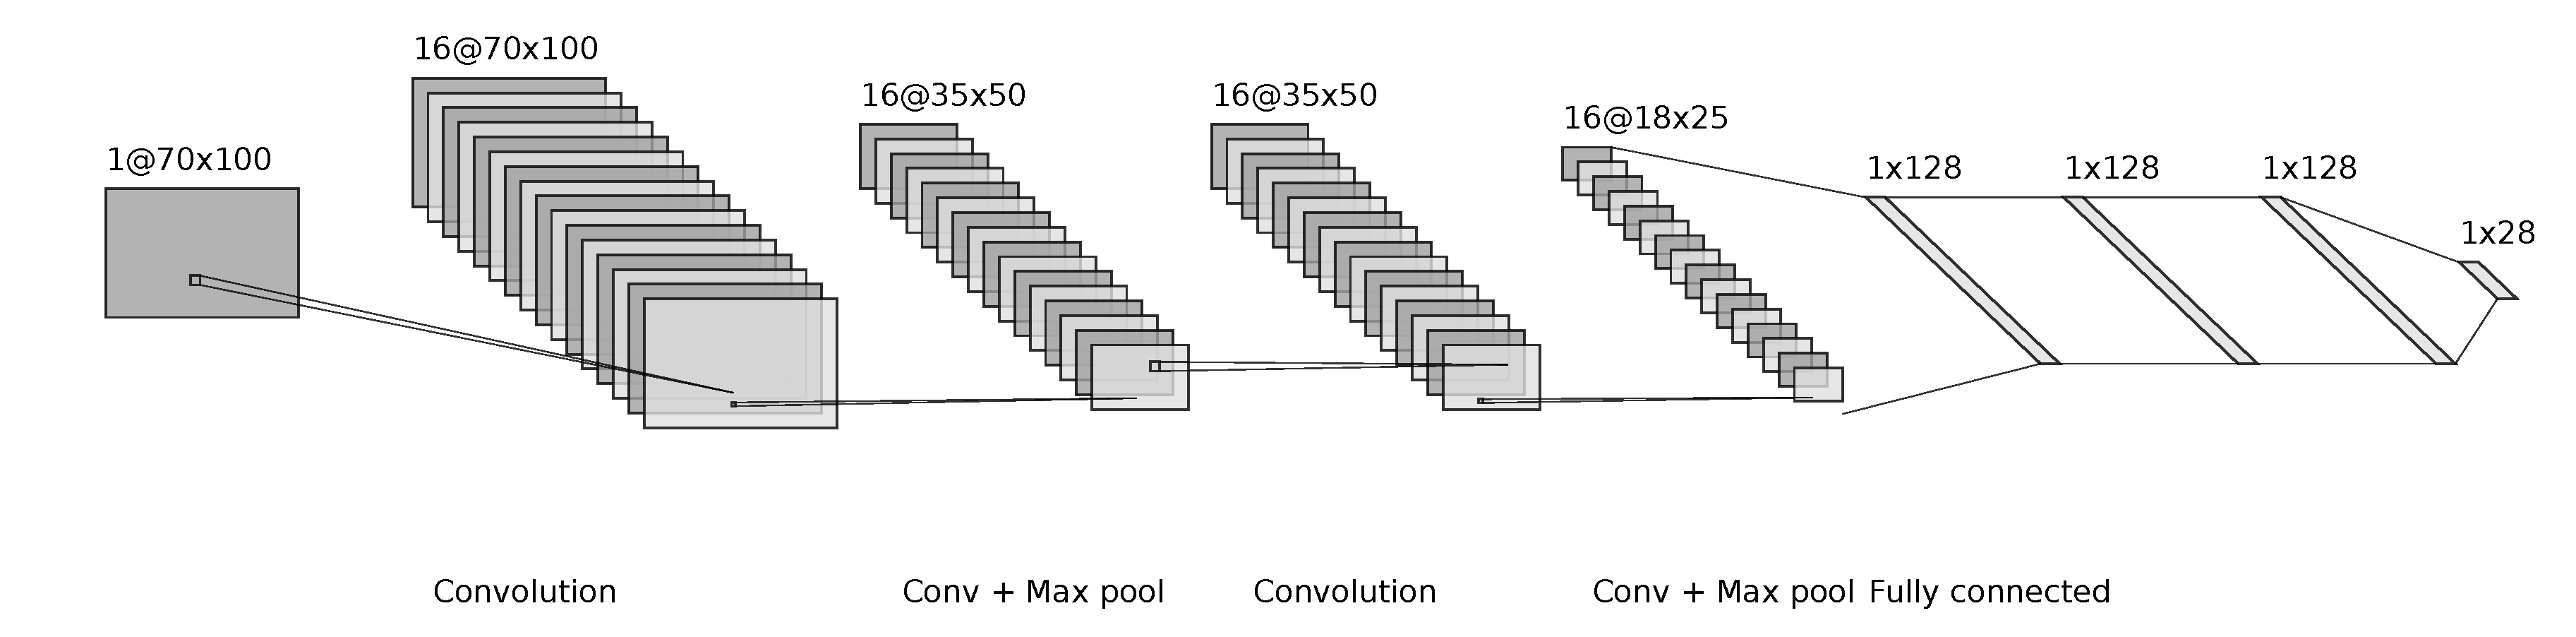
\includegraphics[width=1.1\textwidth]{./images/object_net.pdf}
       \caption{Overview of Convolutional Neural Network Layers}
       \label{fig:cnn}
     \end{center}
\end{figure*}

\subsection{3D CNN experiment}
We experimented with 3D CNN as dataset could be transformed into the
input of 3D CNN being a 3D point cloud dataset. Our approach was to convert point clouds into a set of voxels by voxelization. Voxelization is the process of conversion of a geometric object from its
continuous geometric representation into a set of voxels that best approximates the continuous object.we used the process to fit a bounding box voxel around the point cloud to form a voxel grid. we designed for 4 layered 3D CNN architecture with 2 fully connected layers, a dropout layer, around a softmax layer at the end. The voxel-grid is feed into the network as input and network predict the object out the 28 classes on which network is trained. The 3D CNN model gave the best performance when trained on a minimal number of class attributes but failed to perform when trained on all the class. The major reason we tracked for low performance of 3D CNN with a large number of output classes was the
density of the object and its distribution.
The performance could be improved by experimenting with lower voxel size to increase more voxels for input. This method is high resources dependent as the input size grows from several megabytes to several gigabytes, making harder to work on a standard system. Reviewing the performance between 2D CNN and 3D CNN, the 2D CNN model was providing better performance and precision.
